\section{Exercise name}
In Exercise ..., we are asked to 

..given by the code snippet below.

% \lstinputlisting[linerange={0-112}]{question1.py}

This script produces the following outputs:
% \lstinputlisting[language={}]{q1output.txt}

Our script produces the following figures, see Figure \ref{fig:fig}, and Figure \ref{fig:fig}. From these figures, we see ..


\begin{figure}[ht]
\centering
\begin{minipage}[t]{.5\textwidth}
  \centering
  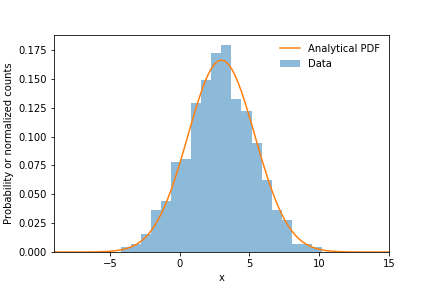
\includegraphics[width=1.0\linewidth]{./plots/q1b1.png}
  \captionsetup{width=0.8\linewidth}
  \captionof{figure}{..}
  \label{fig:fig}
\end{minipage}%
\begin{minipage}[t]{.5\textwidth}
  \centering
  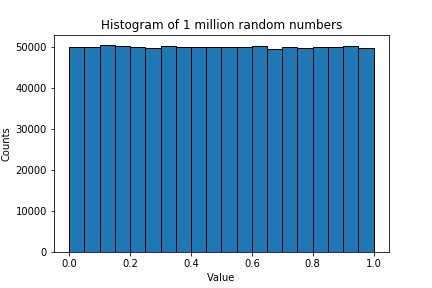
\includegraphics[width=1.0\linewidth]{./plots/q1b2.png}
  \captionsetup{width=0.8\linewidth}
  \captionof{figure}{..}
  \label{fig:fig}
\end{minipage}
\end{figure}

